% PREAMBLE
\documentclass[12pt,a4paper]{book}
\usepackage[inner=2.00cm, outer=2.00cm, top=3.00cm, bottom=3.00cm]{geometry}
\usepackage{subfiles}
\usepackage[utf8]{inputenc}   
\usepackage[main=english,ngerman]{babel}
\usepackage{graphicx}

\usepackage{titlesec}
\titleformat{\chapter}[display]{\Large\bfseries}{\chaptername\ \thechapter}{20pt}{\Large}
\titleformat{\section}{\large\bfseries}{\thesection}{1em}{}
\titleformat{\subsection}{\normalsize\bfseries}{\thesubsection}{1em}{}
\titleformat{\subsubsection}{\small\bfseries}{\thesubsubsection}{1em}{}
\titlespacing*{\chapter}
  {0pt}     % left margin
  {10pt}     % space before (← this moves the chapter up!)
  {20pt}
\usepackage[font=small]{caption}
\usepackage{enumitem}
\renewcommand\labelitemi{$\vcenter{\hbox{\tiny$\bullet$}}$}

\title{Variational Ground States and Quasiparticle Excitations in Isometric Tensor Network States}
\author{Lukas Julius Wittmann}
\date{\today}
\makeatletter
\makeatother

\PassOptionsToPackage{dvipsnames}{xcolor}
\usepackage[most]{tcolorbox} 
\usepackage{hyperref}
\hypersetup{
  colorlinks=true,
  linkcolor=ForestGreen,
  citecolor=ForestGreen,
  urlcolor=ForestGreen,
  pdfborder={0 0 0},
  breaklinks=true, 
  pdfauthor={\@author},
  pdftitle={\@title},
  pdfkeywords={
        Technische Universität München;
        TUM School of Natural Sciences;
        Master's Thesis;
        Lukas Julius Wittmann
    }
}
\definecolor{purple}{RGB}{148, 0, 211}
\colorlet{darkpurple}{purple!70!black}
\definecolor{IntenseLimeGreen}{RGB}{0,170,0}
\definecolor{IntenseCerulean}{RGB}{0,120,220}

\usepackage{bbm}
\usepackage{amsmath}
\allowdisplaybreaks
\usepackage{amsfonts}
\usepackage{amssymb}
\usepackage{physics}
\usepackage{mathtools}
\usepackage{braket}
\newcommand{\tket}[1]{\left| #1 \right)}
\newcommand{\tbra}[1]{\left( #1 \right|}
\DeclareMathOperator*{\argmin}{arg\,min}
\DeclareMathOperator*{\argmax}{arg\,max}
\usepackage{amsthm}
\newcounter{theorem}[chapter]
\renewcommand{\thetheorem}{\thechapter.\arabic{theorem}}
\newtcbtheorem[
  use counter=theorem,
  number within=chapter
]{theorem}{Theorem}{
  enhanced,
  breakable,
  colback=white,
  colframe=blue,
  fonttitle=\bfseries
}{thm}
\renewcommand{\eqref}[1]{(\ref{#1})}

\usepackage[normalem]{ulem}
\usepackage{tikz}
\usepackage{graphicx}
\usepackage{wrapfig}
\usepackage{float}

\usepackage{array}
\usepackage{comment}

%\usepackage{natbib}
\bibliographystyle{alpha}

% BEGIN DOCUMENT
\begin{document}
%\raggedbottom
%\flushbottom

% TITLE PAGE
\thispagestyle{empty}
\newgeometry{left=2cm, right=2cm, top=3.00cm, bottom=3.00cm}
\pagenumbering{gobble}
\vspace{15mm}
\begin{center}
    \LARGE
    \textsc{Variational Ground States \\
    and Quasiparticle Excitations \\
    in Isometric Tensor Network States}
\end{center}
\vspace{4ex}
\begin{center}
    \Large
    Master's Thesis \\
    Quantum Science and Technology \\
    \normalsize
    \vspace{1.5ex}
    Technische Universität München (TUM) and Ludwig-Maximilians-Universität (LMU)
\end{center}
\vspace{4ex}
\begin{center} 
    \Large Lukas Julius Wittmann 
\end{center}
\vfill
\begin{center}
\raisebox{-0.5\height}{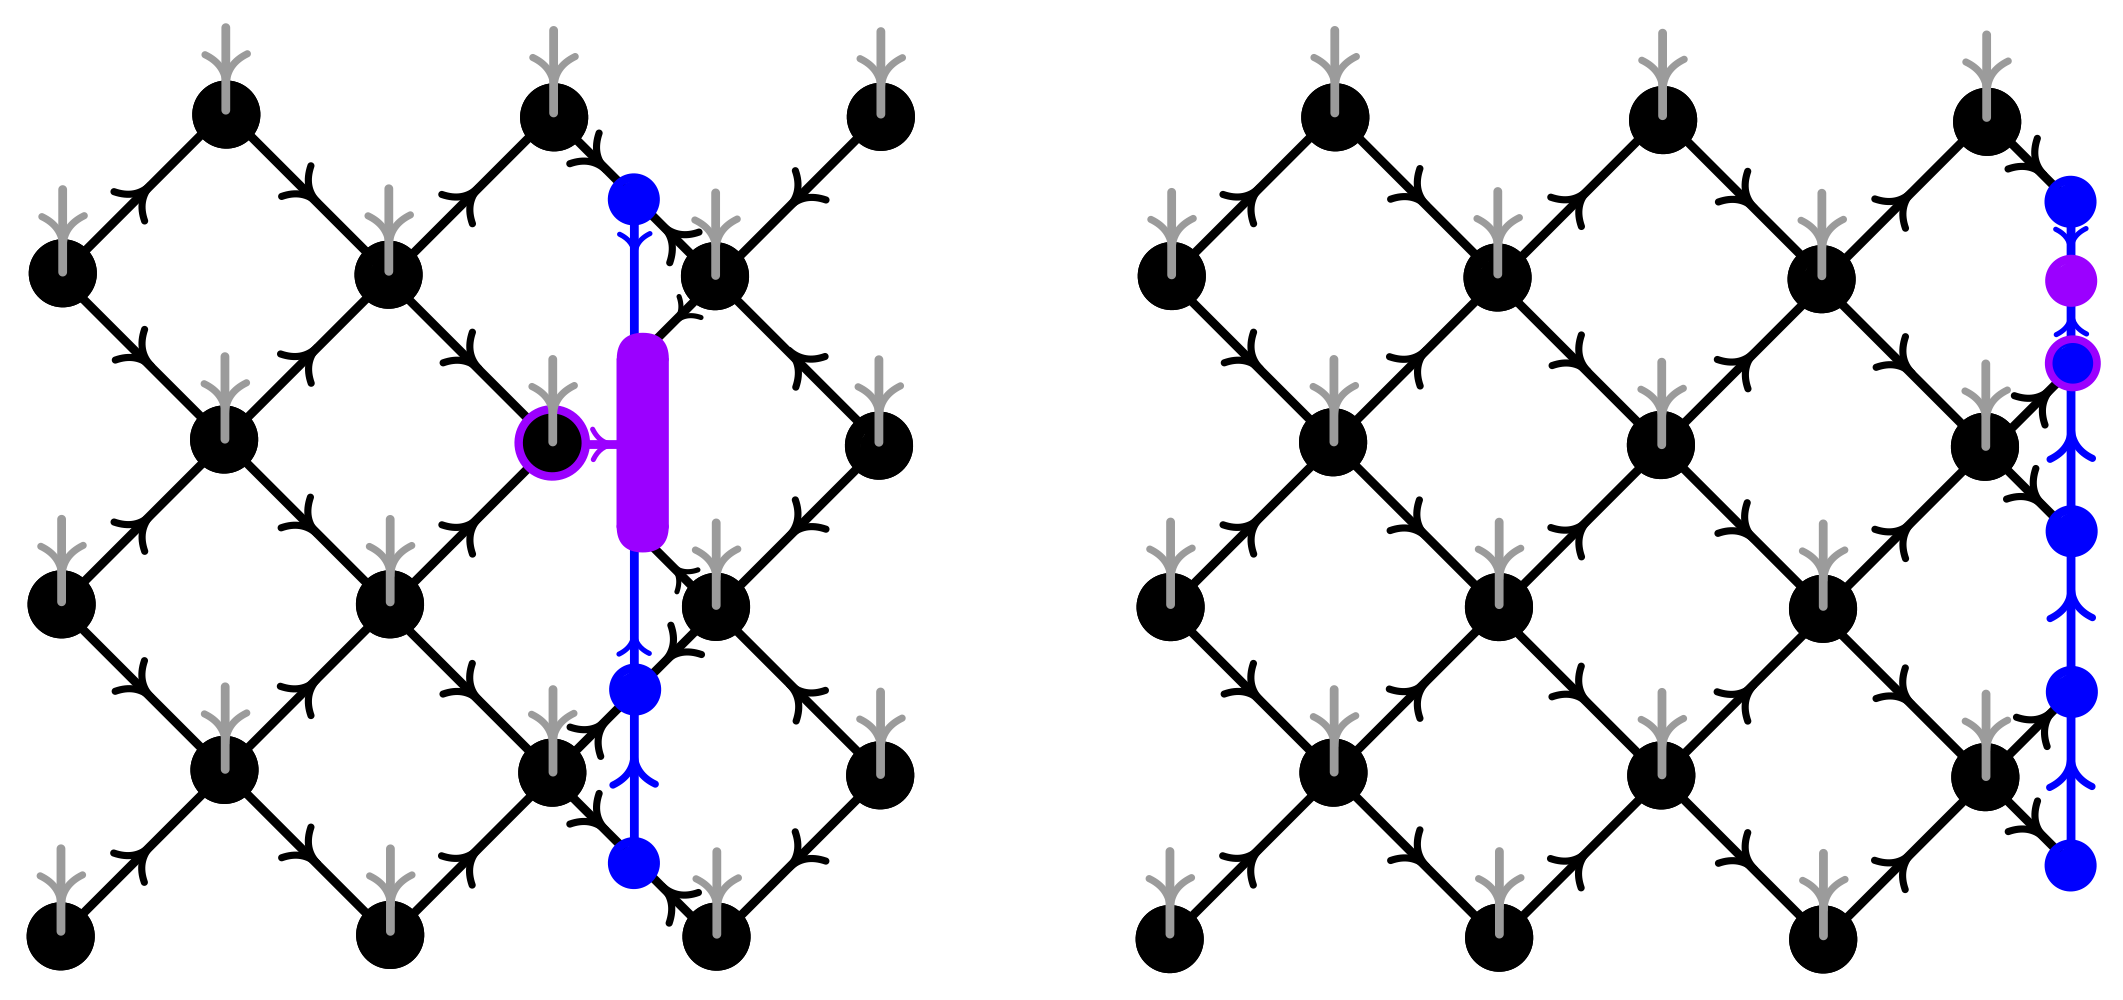
\includegraphics[height=6cm]{title_page/title_pic_2.png}}
\end{center}
\vfill
\begin{center}
    
\includegraphics[height=1cm]{title_page/tum_logo.png}
    \\[2ex]
    Chair of Solid-State Theory
    \\
    TUM School of Natural Sciences, Department of Physics
    \\
    Technical University of Munich
\end{center}
\newpage
\begin{center}
September 2025
\end{center}
\vfill
\begin{center}
Supervisor: Dr. Johannes Hauschild \\
First examiner: Prof. Dr. Frank Pollmann \\
Second examiner: Prof. Dr. Michael Knap
\end{center}
\restoregeometry

% FRONTMATTER
\frontmatter

\chapter{Abstract} 
\label{ch:abstract}
\subfile{frontmatter/a_abstract}

\tableofcontents

% MAINMATTER
\mainmatter

\chapter{Introduction} 
\label{ch:introduction}
\subfile{mainmatter/1_introduction/1_introduction}

\chapter{Transverse field Ising model}
\label{ch:tfi_model}
\subfile{mainmatter/2_tfi_model/2_tfi_model}

\chapter{Tensor network basics}
\label{ch:tensor_networks}
\subfile{mainmatter/3_tensor_network_basics/3_tensor_network_basics}

\chapter{Uniform matrix product states (uMPS)} 
\label{ch:umps}
\subfile{mainmatter/4_umps/4_umps}

\chapter{Matrix product states (MPS)} 
\label{ch:mps}
\subfile{mainmatter/5_mps/5_mps}

\chapter{Isometric projected entangled pair states (isoPEPS)} \label{ch:iso_peps}
\subfile{mainmatter/6_iso_peps/6_iso_peps}

\chapter{Conclusion and outlook}
\label{ch:conclusion}
\subfile{mainmatter/7_conclusion/7_conclusion}

% APPENDIX
\appendix

\chapter{Detailed Jordan-Wigner and Bogoliubov transformation} \label{ch:detailed_tfi_solution}
\subfile{appendix/a_detailed_tfi_solution}

\chapter{Quantum channels and matrix product states} \label{ch:quantum_channels_mps}
\subfile{appendix/b_quantum_channels_mps/b_quantum_channels_mps}

\chapter{Extensive tensor network diagrams}
\label{ch:extensive_tensor_network_diagrams}
\subfile{appendix/c_extended_tensor_network_diagrams/c_extended_tensor_network_diagrams}

% BACKMATTER
\backmatter
\bibliography{thesis}
\addcontentsline{toc}{chapter}{Bibliography}

% END DOCUMENT
\end{document}
